\documentclass{lab_sheet}
\usepackage{hyperref}
\def\ddfrac#1#2{\displaystyle\frac{\displaystyle #1}{\displaystyle #2}}

\newcommand{\outputWindow}[2]{
    \begin{figure}[H]
        \centering
        \includegraphics[width=0\linewidth]{../Figures/#1-#2.eps}
        \caption{Plot for #1-point symmetric #2 window}
        \label{fig:#1-#2}
    \end{figure}
    \begin{figure}[H]
        \centering
        \includegraphics[width=0.65\linewidth]{../Figures/#1-#2-resp.eps}
        \caption{Plot for frequency response for #2 window function with M=#1} 
        \label{fig:#1-#2-window}
    \end{figure}
    \begin{figure}[H]
        \centering
        \includegraphics[width=0.65\linewidth]{../Figures/#1-#2-fir.eps}
        \caption{Plot for frequency response for FIR filter using #2 window for M=#1}
        \label{fig:#1-#2-fir}
    \end{figure}
    \pagebreak
}
\begin{document}
\titlePage{Design of FIR Digital Filters using Window method}{January 30, 2022}
\pagenumbering{roman}
\clearpage
\tableofcontents
\clearpage
\phantomsection
\addcontentsline{toc}{section}{\bfseries{List of Figures}}
\listoffigures
\clearpage
\phantomsection
\addcontentsline{toc}{section}{\bfseries{Listings}}
\lstlistoflistings
\clearpage
\pagenumbering{arabic}
\section{Objectives}
\begin{itemize}
	\item Familiarization with design of FIR digital filters using window method.
	\item Comparison of response for designed FIR filters with different window functions.
\end{itemize}
\section{Background Theory}
In previous experiment we discussed the most commonly used techniques for design of IIR filters based on transformations of continuous-time IIR systems into discrete time IIR systems. The major difficulty lies in the implementation of the non-iterative direct design method for IIR filters. However FIR filters are almost entirely restricted to discrete-time implementations. Thus the design techniques for FIR filters are based on directly approximating the desired frequency response of the discrete time system. Furthermore, most techniques for approximating the magnitude response of the FIR system assume a linear phase constraint; thereby avoiding the problem of spectrum factorization that complicates the direct design of IIR filters.\\ 
The simplest method of FIR design is called the window method. This method generally begins with an ideal desired frequency response $H_d(\omega)$. The impulse response $h_d(n)$ of the filter exhibiting this desired frequency response can be obtained from inverse Fourier transform of $H_d(\omega)$. However this impulse response exists for $n=-\infty$ to $+\infty$ and hence truncation is needed to make the finite duration impulse response. The truncation is similar to the multiplication of the $h_d(n)$ with the window function $w(n)$. The multiplication in discrete time domain is equivalent to the convolution of the two in frequency domain, which actually gives the frequency response of the truncated FIR filter.\\
But depending on the tapering of the window to zero at each end, the nature of the window differs. For example, the rectangular window exhibits the most abrupt changes while approaching to zero at each end. For the specific value of length of the window, the rectangular window exhibits main lobe with the greatest width and the lowest side lobe attenuation, than the other windows like Bartlett, Hanning, Hamming, Blackman etc. There are also adjustable windows like Kaiser windows whose windowing function $w(n)$ can be adjusted by changing the value of parameter $\beta$ according to the stop band attenuation $A$ as given below,
\begin{equation*}
    \beta=\begin{cases}
        0.1102(A-8.7)\quad &\text{if }A>50\\
        0.5842(A-0.21)^{0.4}+0.07886(A-21)\quad &\text{if }21\leq A \leq 50\\
        0.0 \quad &\text{if }A<21
    \end{cases}
\end{equation*}
where $A=-20\log_{10}\delta$. The length of the Kaiser window is given by,
\begin{equation*}
    M=\ddfrac{\delta-7.95}{14.36\Delta\omega}+1,\quad \text{where }\Delta\omega=\ddfrac{\omega_s-\omega_p}{2}
\end{equation*}
To determine and plot the different types of windowing functions and their frequency responses, built-in functions like \texttt{Bartlett}, \texttt{Hamming}, \texttt{Hanning}, \texttt{Blackman}, \texttt{Kaiser} etc. are available. There is a function \texttt{fir1} that can be used to obtain the frequency response of the designed FIR filter. Use MATLAB \texttt{help} for further information of the functions.
\section{Lab Exercises}
\mysub{Design of FIR filter with window functions}
\problem{Design an FIR linear phase digital filter approximating the ideal frequency response}
\begin{equation*}
    H(\omega)=\begin{cases}
        1,\quad &\text{for }|\omega| \leq \ddfrac{\pi}{6}\\
        0, \quad & \text{for } \ddfrac{\pi}{6}<|\omega|\leq\pi
    \end{cases}
\end{equation*}
\subproblem{a. Plot the window function for Hamming and its frequency response for length of $M=31$.}
\subproblem{b. Using the Hamming window plot the frequency response of the truncated FIR filter.}
\subproblem{c. Repeat parts (a) and (b) for the Hanning, Blackman and Bartlett windows.}
\pagebreak
\subproblem{d. Repeat parts (a), (b) and (c) for filter length of $M=61$.}
\matlabcode{window_selector}{Matlab function to select particular window function based on user input}
\matlabcode{freqRespPlot}{Matlab function to plot the frequency response for given \texttt{H} and \texttt{w} and return the main lobe width and relative side lobe attenuation}
\matlabcode{lab_6_1}{Matlab script for visualizing window function and frequency responses of the window function and the designed truncated FIR filter}
\pagebreak
\mysubsub{Hamming Window (M=31)}
\begin{verbatim}
    >> lab_6_1
    Enter the type of window: hamming
    Enter the value of M: 31
    Parameters for FIR filter using hamming window:
    Main lobe width = 0.281
    Relative side lobe attenuation = -52.126
\end{verbatim}
\outputWindow{31}{hamming}

\mysubsub{Hanning Window}
\begin{verbatim}
    >> lab_6_1
    Enter the type of window: hanning
    Enter the value of M: 31
    Parameters for FIR filter using hanning window:
    Main lobe width = 0.279
    Relative side lobe attenuation = -43.887
\end{verbatim}
\outputWindow{31}{hanning}

\mysubsub{Blackman Window}
\begin{verbatim}
    >> lab_6_1
    Enter the type of window: blackman
    Enter the value of M: 31
    Parameters for FIR filter using blackman window:
    Main lobe width = 0.266
    Relative side lobe attenuation = -74.275
\end{verbatim}
\outputWindow{31}{blackman}

\mysubsub{Bartlett Window}
\begin{verbatim}
    >> lab_6_1
    Enter the type of window: bartlett
    Enter the value of M: 31
    Parameters for FIR filter using bartlett window:
    Main lobe width = 0.285
    Relative side lobe attenuation = -28.025
\end{verbatim}
\outputWindow{31}{bartlett}

\begin{verbatim}
    >> lab_6_1
    Enter the type of window: hamming
    Enter the value of M: 61
    Parameters for FIR filter using hamming window:
    Main lobe width = 0.307
    Relative side lobe attenuation = -51.966
\end{verbatim}
\outputWindow{61}{hamming}

\begin{verbatim}
    >> lab_6_1
    Enter the type of window: hanning
    Enter the value of M: 61
    Parameters for FIR filter using hanning window:
    Main lobe width = 0.307
    Relative side lobe attenuation = -44.021
\end{verbatim}
\outputWindow{61}{hanning}

\begin{verbatim}
    >> lab_6_1
    Enter the type of window: blackman
    Enter the value of M: 61
    Parameters for FIR filter using blackman window:
    Main lobe width = 0.299
    Relative side lobe attenuation = -75.617
\end{verbatim}
\outputWindow{61}{blackman}

\begin{verbatim}
    >> lab_6_1
    Enter the type of window: bartlett
    Enter the value of M: 61
    Parameters for FIR filter using bartlett window:
    Main lobe width = 0.309
    Relative side lobe attenuation = 
\end{verbatim}
\outputWindow{61}{bartlett}

\mysub{Comparison of effects of different windowing functions on frequency response of FIR filter}
\problem{Discuss the effects of different types of the windowing functions on the frequency response of the FIR filter. Carry out the comparative study on the basis of the peak side lobe level, the approximate transition width of the main lobe etc. Also discuss on the effects of increasing value of M.}
The frequency response of each designed FIR filter with different window functions, namely, hamming, hanning, blackman, bartlett are observed in the Figures above. The parameters such as the main lobe width and the relative side lobe attenuation are also determined and printed in the command console in MATLAB. It can be observed that the fourier transforms of the windows are generally concentrated at $\omega=0$, which in fact is the desired property. In comparison, the different window responses have varying main lobe width and relative side lobe attenuation, among which there is a trade off. This tradeoff is distinctly visible in blackman window that has the main lobe width of approximately $0.266 (\times \pi \text{ rad/samples})$  and the relative side lobe attenuation is $-74.275$ dB. Likewise, for bartlett window, the side lobe level is increased with narrower main lobe width. By increasing the value of $M$, the main lobe width increases along with increased number of side lobes.

\mysub{Design of FIR filter using Kaiser and Hamming with given specifications}
\problem{An analog signal $x(t)$ consists of the sum of two components $x_1(t)$ and $x_2(t)$. The spectral characteristics of $x(t)$ is shown in Figure. The signal $x(t)$ is band limited to $40 \text{ kHz}$ and is
sampled at the rate of $100 \text{ kHz}$ to yield the sequence $x(n)$}
\begin{figure}[H]
    \centering
    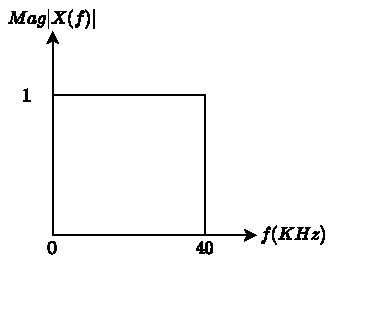
\includegraphics[]{../Figures/fig_3.pdf}
\end{figure}
\subproblem{It is desired to suppress the signal $x_2(t)$ by passing the sequence $x(n)$ through a digital low pass filter. The allowable distortion on $|X_1(f)|$ is $\pm2\%$ $(\delta_1=0.02)$ over the range $0\leq|F|\leq 15 \text{ kHz}$. Above $20 \text{ kHz}$, the filter must have an attenuation of at least $40 \text{ dB} (\delta_2=0.01)$.}
\subproblem{a. For obtaining the filter with above specifications, use the Kaiser window and determine the length of the required window. Plot the frequency response of the filter and its impulse response also.}
\subproblem{b. If the same filter is to be designed using Hamming window what would be the length of the required window. Plot the frequency and impulse response of the filter.}

\matlabcode{betaValue}{Matlab function to return the value of $\beta$ based on the attenuation $A$}
\matlabcode{lab_6_3}{Matlab script for visualizing the frequency response of designed FIR filter from either kaiser or hamming window based on user input}
\begin{verbatim}
    >> lab_6_3
    Enter the type of window: kaiser
    Parameters for FIR filter using kaiser window:
    Window length: 47
    Main lobe width = 0.672
    Relative side lobe attenuation = -40.228
\end{verbatim}

\begin{figure}[H]
    \centering
    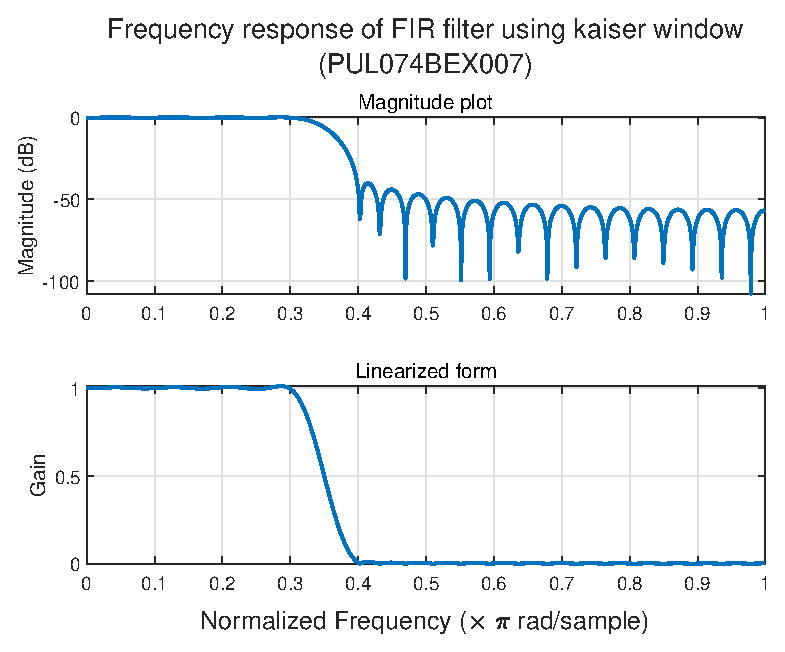
\includegraphics[width=0.65\linewidth]{../Figures/kaiser-fir.eps}
    \caption{Plot for frequency response for FIR filter using kaiser window for M=47}
    \label{fig:kaiser-fir}
\end{figure}

\begin{figure}[H]
    \centering
    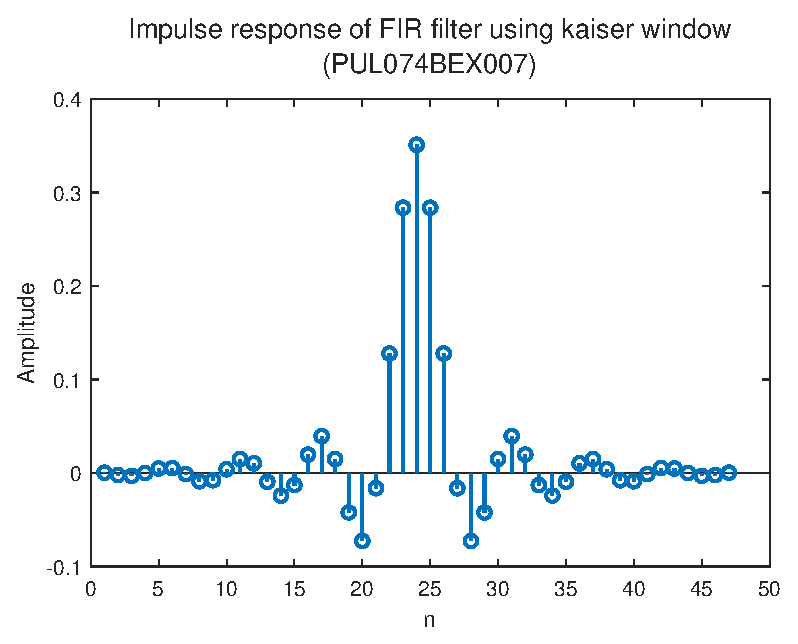
\includegraphics[width=0.65\linewidth]{../Figures/kaiser-imp.eps}
    \caption{Plot for impulse response for FIR filter using kaiser window for M=47}
    \label{fig:kaiser-imp}
\end{figure}
\pagebreak
\begin{verbatim}
    >> lab_6_3
    Enter the type of window: hamming
    Parameters for FIR filter using hamming window:
    Window length: 61
    Main lobe width = 0.674
    Relative side lobe attenuation = -54.289
\end{verbatim}

\begin{figure}[H]
    \centering
    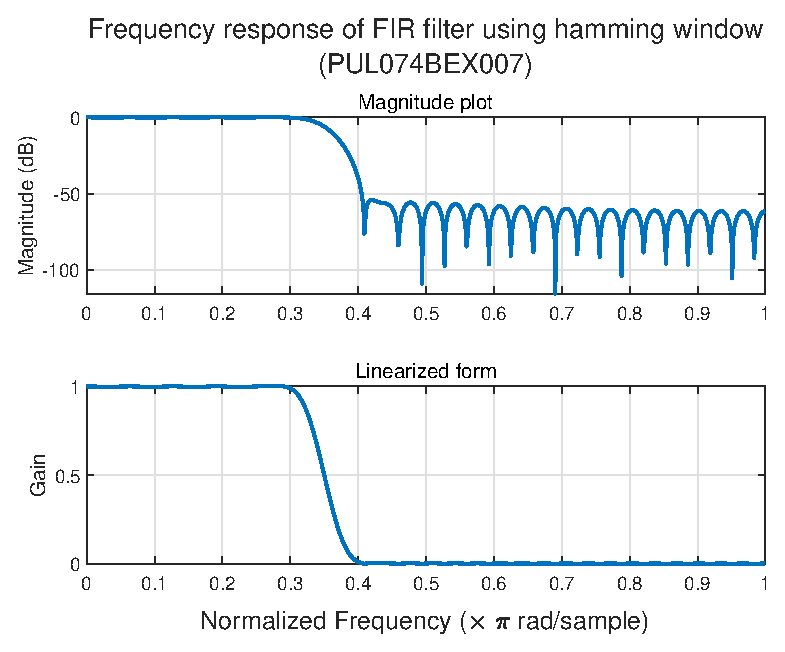
\includegraphics[width=0.65\linewidth]{../Figures/hamming-fir.eps}
    \caption{Plot for frequency response for FIR filter using hamming window for M=61}
    \label{fig:hamming-fir}
\end{figure}

\begin{figure}[H]
    \centering
    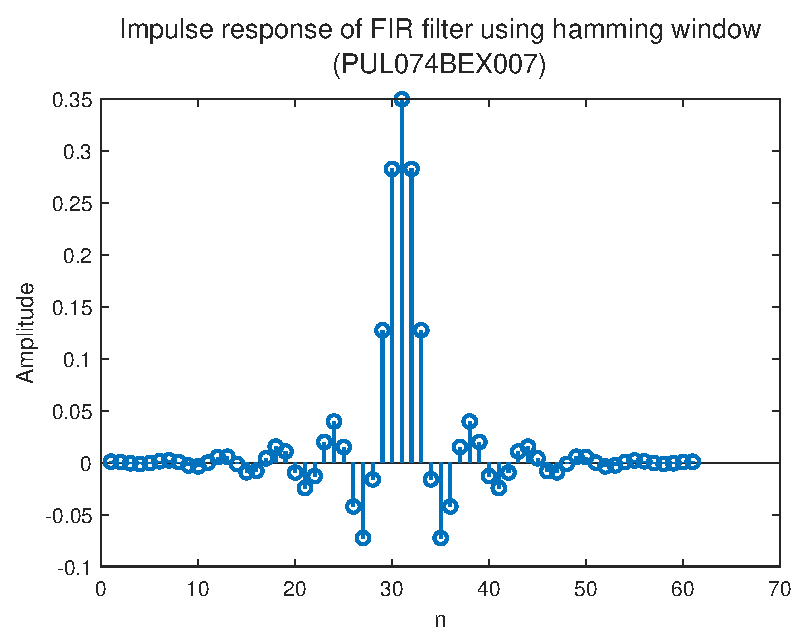
\includegraphics[width=0.65\linewidth]{../Figures/hamming-imp.eps}
    \caption{Plot for impulse response for FIR filter using hamming window for M=61}
    \label{fig:hamming-imp}
\end{figure}

\section{Discussion and Conclusion}
In this lab experiment we dealt with the design and analysis of FIR filters using various windowing functions. Firstly, a window function such as Hamming, Hanning, Blackman, Bartlett or Kaiser is used to get the desired window function. The window functions like \texttt{Hamming}, \texttt{Hanning}, \texttt{Blackman}, \texttt{Bartlett}, \texttt{Kaiser} etc. are used to return the window function. Then the \texttt{fir1} function is used to obtain the frequency response of the designed FIR filter. The frequency responses of the window function, and designed FIR filter are plotted and analysis of parameters such as the main lobe width and relative side lobe attenuation is performed. The effect of increasing the window length was also noted on these parameters and the responses were plotted. Lastly, a kaiser window was used to design a FIR filter at given requirements. The value of $\beta$, which in fact is a function of attenuation $A$ was used to return the window function to be used. The length of kaiser window was calculated to be M=47. An equivalent design using the hamming window for M=61 was attempted. \\
Hence, the objectives of the lab experiment were fulfilled.
\end{document}
